\documentclass{standalone}
\usepackage{tikz}
\usetikzlibrary{patterns, positioning}


\begin{document}
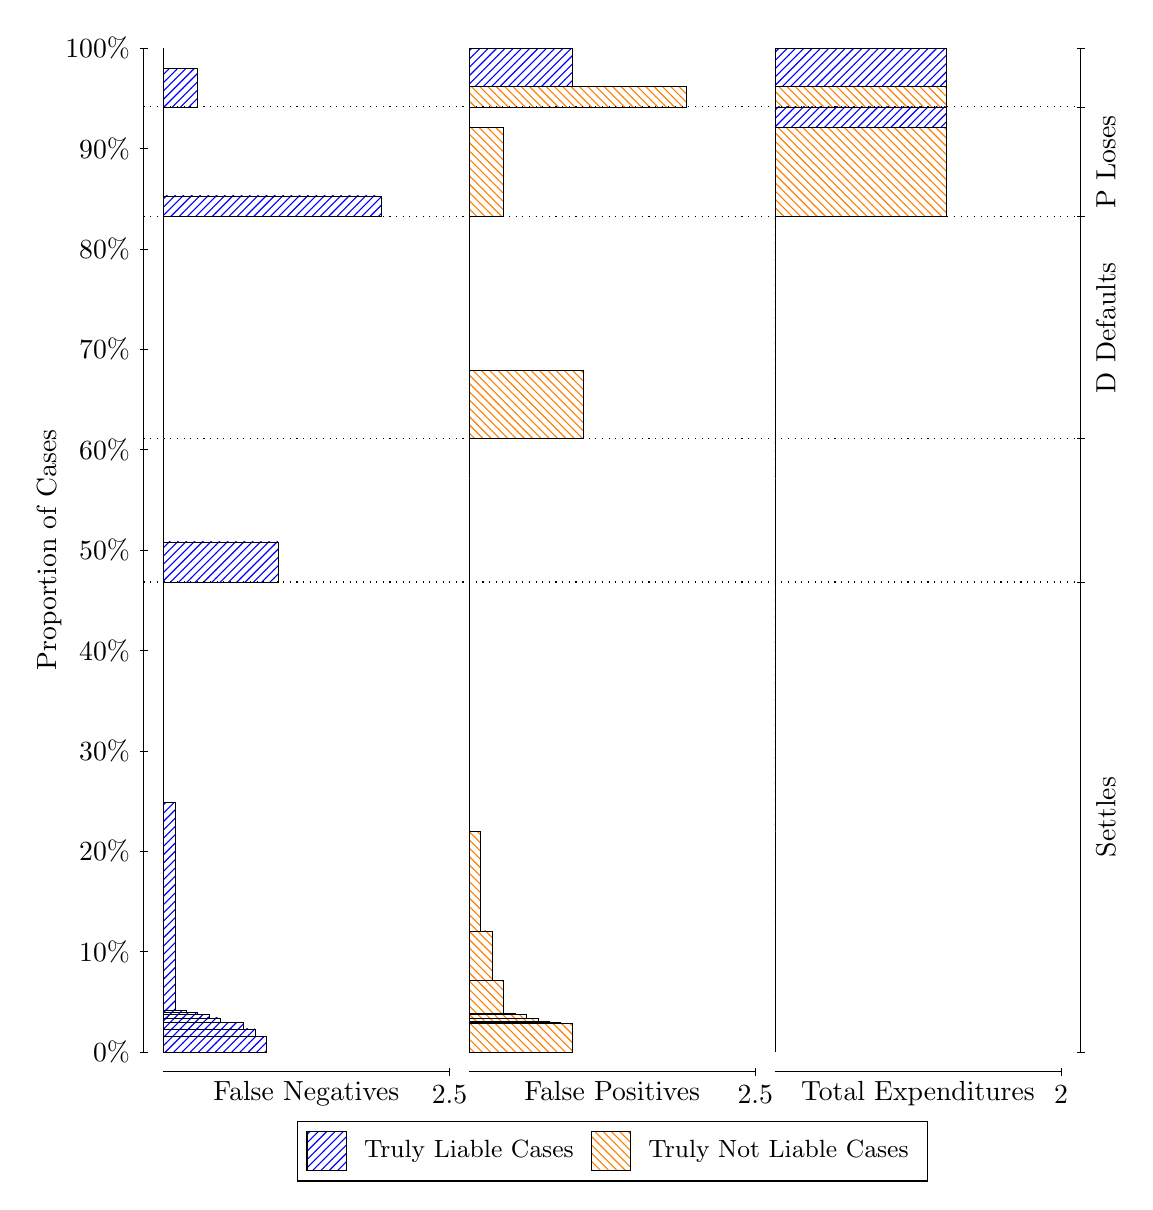
\begin{tikzpicture}
\draw[black, very thin] (1.5,1.75) -- (1.5,14.5);
\node[rotate=90, text=black, anchor=center] at (0.3, 8.125) {Proportion of Cases};
\draw[black, very thin] (1.45,1.75) -- (1.55,1.75);
\node[text=black, anchor=east] at (1.45, 1.75) {0\%};
\draw[black, very thin] (1.45,3.025) -- (1.55,3.025);
\node[text=black, anchor=east] at (1.45, 3.025) {10\%};
\draw[black, very thin] (1.45,4.3) -- (1.55,4.3);
\node[text=black, anchor=east] at (1.45, 4.3) {20\%};
\draw[black, very thin] (1.45,5.575) -- (1.55,5.575);
\node[text=black, anchor=east] at (1.45, 5.575) {30\%};
\draw[black, very thin] (1.45,6.85) -- (1.55,6.85);
\node[text=black, anchor=east] at (1.45, 6.85) {40\%};
\draw[black, very thin] (1.45,8.125) -- (1.55,8.125);
\node[text=black, anchor=east] at (1.45, 8.125) {50\%};
\draw[black, very thin] (1.45,9.4) -- (1.55,9.4);
\node[text=black, anchor=east] at (1.45, 9.4) {60\%};
\draw[black, very thin] (1.45,10.675) -- (1.55,10.675);
\node[text=black, anchor=east] at (1.45, 10.675) {70\%};
\draw[black, very thin] (1.45,11.95) -- (1.55,11.95);
\node[text=black, anchor=east] at (1.45, 11.95) {80\%};
\draw[black, very thin] (1.45,13.225) -- (1.55,13.225);
\node[text=black, anchor=east] at (1.45, 13.225) {90\%};
\draw[black, very thin] (1.45,14.5) -- (1.55,14.5);
\node[text=black, anchor=east] at (1.45, 14.5) {100\%};

\draw[black, very thin] (13.4,1.75) -- (13.4,14.5);
\draw[black, very thin] (13.35,1.75) -- (13.45,1.75);
\node[anchor=west] at (13.35, 1.75) {};
\draw[black, very thin] (13.35,7.7191) -- (13.45,7.7191);
\node[anchor=west] at (13.35, 7.7191) {};
\draw[black, very thin] (13.35,9.5394) -- (13.45,9.5394);
\node[anchor=west] at (13.35, 9.5394) {};
\draw[black, very thin] (13.35,12.359) -- (13.45,12.359);
\node[anchor=west] at (13.35, 12.359) {};
\draw[black, very thin] (13.35,13.753) -- (13.45,13.753);
\node[anchor=west] at (13.35, 13.753) {};
\draw[black, very thin] (13.35,14.5) -- (13.45,14.5);
\node[anchor=west] at (13.35, 14.5) {};

\draw[black, very thin, pattern color=blue, pattern=north east lines] (1.75,1.75) rectangle (3.058,1.9454);
\draw[black, very thin, pattern color=blue, pattern=north east lines] (1.75,1.9454) rectangle (2.9127,2.0427);
\draw[black, very thin, pattern color=blue, pattern=north east lines] (1.75,2.0427) rectangle (2.7673,2.1214);
\draw[black, very thin, pattern color=blue, pattern=north east lines] (1.75,2.1214) rectangle (2.622,2.1258);
\draw[black, very thin, pattern color=blue, pattern=north east lines] (1.75,2.1258) rectangle (2.622,2.1292);
\draw[black, very thin, pattern color=blue, pattern=north east lines] (1.75,2.1292) rectangle (2.4767,2.1838);
\draw[black, very thin, pattern color=blue, pattern=north east lines] (1.75,2.1838) rectangle (2.3313,2.231);
\draw[black, very thin, pattern color=blue, pattern=north east lines] (1.75,2.231) rectangle (2.186,2.2536);
\draw[black, very thin, pattern color=blue, pattern=north east lines] (1.75,2.2536) rectangle (2.0407,2.277);
\draw[black, very thin, pattern color=blue, pattern=north east lines] (1.75,2.277) rectangle (1.8953,4.9168);
\draw[black, very thin, pattern color=orange, pattern=north west lines] (1.75,4.9168) rectangle (1.75,7.7191);
\draw[black, very thin, pattern color=blue, pattern=north east lines] (1.75,7.7191) rectangle (3.2033,8.2277);
\draw[black, very thin, pattern color=orange, pattern=north west lines] (1.75,8.2277) rectangle (1.75,9.5394);
\draw[black, very thin, pattern color=orange, pattern=north west lines] (1.75,9.5394) rectangle (1.75,10.41);
\draw[black, very thin, pattern color=blue, pattern=north east lines] (1.75,10.41) rectangle (1.75,12.359);
\draw[black, very thin, pattern color=blue, pattern=north east lines] (1.75,12.359) rectangle (4.5113,12.622);
\draw[black, very thin, pattern color=orange, pattern=north west lines] (1.75,12.622) rectangle (1.75,13.753);
\draw[black, very thin, pattern color=blue, pattern=north east lines] (1.75,13.753) rectangle (2.186,14.24);
\draw[black, very thin, pattern color=orange, pattern=north west lines] (1.75,14.24) rectangle (1.75,14.5);
\draw[black, very thin, pattern color=orange, pattern=north west lines] (5.6333,1.75) rectangle (6.9413,2.1165);
\draw[black, very thin, pattern color=orange, pattern=north west lines] (5.6333,2.1165) rectangle (6.796,2.1266);
\draw[black, very thin, pattern color=orange, pattern=north west lines] (5.6333,2.1266) rectangle (6.6507,2.1375);
\draw[black, very thin, pattern color=orange, pattern=north west lines] (5.6333,2.1375) rectangle (6.5053,2.1741);
\draw[black, very thin, pattern color=orange, pattern=north west lines] (5.6333,2.1741) rectangle (6.36,2.2278);
\draw[black, very thin, pattern color=orange, pattern=north west lines] (5.6333,2.2278) rectangle (6.2147,2.2346);
\draw[black, very thin, pattern color=orange, pattern=north west lines] (5.6333,2.2346) rectangle (6.2147,2.2442);
\draw[black, very thin, pattern color=orange, pattern=north west lines] (5.6333,2.2442) rectangle (6.0693,2.66);
\draw[black, very thin, pattern color=orange, pattern=north west lines] (5.6333,2.66) rectangle (5.924,3.2886);
\draw[black, very thin, pattern color=orange, pattern=north west lines] (5.6333,3.2886) rectangle (5.7787,4.5523);
\draw[black, very thin, pattern color=blue, pattern=north east lines] (5.6333,4.5523) rectangle (5.6333,7.7191);
\draw[black, very thin, pattern color=orange, pattern=north west lines] (5.6333,7.7191) rectangle (5.6333,9.0309);
\draw[black, very thin, pattern color=blue, pattern=north east lines] (5.6333,9.0309) rectangle (5.6333,9.5394);
\draw[black, very thin, pattern color=orange, pattern=north west lines] (5.6333,9.5394) rectangle (7.0867,10.41);
\draw[black, very thin, pattern color=blue, pattern=north east lines] (5.6333,10.41) rectangle (5.6333,12.359);
\draw[black, very thin, pattern color=orange, pattern=north west lines] (5.6333,12.359) rectangle (6.0693,13.489);
\draw[black, very thin, pattern color=blue, pattern=north east lines] (5.6333,13.489) rectangle (5.6333,13.753);
\draw[black, very thin, pattern color=orange, pattern=north west lines] (5.6333,13.753) rectangle (8.3947,14.013);
\draw[black, very thin, pattern color=blue, pattern=north east lines] (5.6333,14.013) rectangle (6.9413,14.5);
\draw[black, very thin, pattern color=orange, pattern=north west lines] (9.5167,1.75) rectangle (9.5167,4.5523);
\draw[black, very thin, pattern color=blue, pattern=north east lines] (9.5167,4.5523) rectangle (9.5167,7.7191);
\draw[black, very thin, pattern color=orange, pattern=north west lines] (9.5167,7.7191) rectangle (9.5167,9.0309);
\draw[black, very thin, pattern color=blue, pattern=north east lines] (9.5167,9.0309) rectangle (9.5167,9.5394);
\draw[black, very thin, pattern color=orange, pattern=north west lines] (9.5167,9.5394) rectangle (9.5167,10.41);
\draw[black, very thin, pattern color=blue, pattern=north east lines] (9.5167,10.41) rectangle (9.5167,12.359);
\draw[black, very thin, pattern color=orange, pattern=north west lines] (9.5167,12.359) rectangle (11.697,13.489);
\draw[black, very thin, pattern color=blue, pattern=north east lines] (9.5167,13.489) rectangle (11.697,13.753);
\draw[black, very thin, pattern color=orange, pattern=north west lines] (9.5167,13.753) rectangle (11.697,14.013);
\draw[black, very thin, pattern color=blue, pattern=north east lines] (9.5167,14.013) rectangle (11.697,14.5);
\draw[black, dotted] (1.5,7.7191) -- (13.4,7.7191);
\draw[black, dotted] (1.5,9.5394) -- (13.4,9.5394);
\draw[black, dotted] (1.5,12.359) -- (13.4,12.359);
\draw[black, dotted] (1.5,13.753) -- (13.4,13.753);
\draw[black, very thin] (1.75,1.5) -- (5.3833,1.5);
\node[text=black, anchor=north] at (3.5667, 1.5) {False Negatives};
\draw[black, very thin] (5.3833,1.45) -- (5.3833,1.55);
\node[text=black, anchor=north] at (5.3833, 1.45) {2.5};

\draw[black, very thin] (5.6333,1.5) -- (9.2667,1.5);
\node[text=black, anchor=north] at (7.45, 1.5) {False Positives};
\draw[black, very thin] (9.2667,1.45) -- (9.2667,1.55);
\node[text=black, anchor=north] at (9.2667, 1.45) {2.5};

\draw[black, very thin] (9.5167,1.5) -- (13.15,1.5);
\node[text=black, anchor=north] at (11.333, 1.5) {Total Expenditures};
\draw[black, very thin] (13.15,1.45) -- (13.15,1.55);
\node[text=black, anchor=north] at (13.15, 1.45) {2};

\node[text=black, centered, rotate=90] at (13.72, 4.7345) {Settles};

\node[text=black, centered, rotate=90] at (13.72, 10.949) {D Defaults};
\node[text=black, centered, rotate=90] at (13.72, 13.056) {P Loses};


\draw (7.449999999999999,1.5) node[draw=none] (baseCoordinate) {};
\begin{scope}[align=center]
        \matrix[scale=0.5, draw=black, below=0.5cm of baseCoordinate, nodes={draw}, column sep=0.1cm]{
            \node[rectangle, draw, minimum width=0.5cm, minimum height=0.5cm, pattern color=blue, pattern=north east lines] {}; &
            \node[draw=none, font=\small, text=black] (B) {Truly Liable Cases}; &
            \node[rectangle, draw, minimum width=0.5cm, minimum height=0.5cm, pattern color=orange, pattern=north west lines] {}; &
            \node[draw=none, font=\small, text=black] (B) {Truly Not Liable Cases}; \\
            };
\end{scope}

\end{tikzpicture}
\end{document}